%! Author = melek
%! Date = 9.06.2022

% Preamble
\documentclass[11pt]{article}

% Packages
\usepackage{amsmath}
\DeclareMathOperator*{\argmax}{argmax}

\usepackage{graphicx}
\usepackage{amssymb}
\graphicspath{ {../images/} }

% Document
\begin{document}

    \maketitle
    \setcounter{section}{6}


    \section{Exercises}

    \subsection{Question}

    In Chapter 6 we noted that the Monte Carlo error can be written as the sum of TD errors (6.6) if the value estimates don’t change from step to step.
    Show that the n-step error used in (7.2) can also be written as a sum TD errors (again if the value estimates don’t change) generalizing the earlier result.

    \subsection*{Answer}

    Value estimates are assumed not to change thus we can omit value estimate subscripts such that $ V_t(S_t) = V_{t+1}(S_t)$.

    n-step TD Error used in 7.2  is:
    \newline
    $G_{t:t+n} - V(S_t) = R_{t+1} + \gamma G_{t+1:t+n} - V(S_t) $
    \newline
    $G_{t:t+n} - V(S_t) = R_{t+1} + \gamma V(S_{t+1}) - V(S_t) + \gamma G_{t+1:t+n} - \gamma V(S_{t+1}) $
    \newline
    $G_{t:t+n} - V(S_t) = \delta_t + \gamma ( G_{t+1:t+n} - V(S_{t+1}) ) $
    \newline
    $G_{t:t+n} - V(S_t) = \delta_t + \gamma \delta_{t+1} + \gamma^2 ( G_{t+2:t+n} - V(S_{t+2}) ) $
    \newline
    $G_{t:t+n} - V(S_t) = \sum_{k=t}^{t+n-1} \gamma^{k-t} \delta_k  $

    \subsection{Question}

    (programming) With an n-step method, the value estimates do change from step to step, so an algorithm that used the sum of TD errors (see previous exercise) in place of the error in (7.2) would actually be a slightly different algorithm.
    Would it be a better algorithm or a worse one?
    Devise and program a small experiment to answer this question empirically.

    \subsection*{Answer}

    The chart above shows regular n-step TD with different n parameters.
    The chart below shows the same configuration with unchanged value functions.
    Value function updates are applied only after an episode terminates.

    Using sum of TD errors as in place of the error in 7.2 performs worse in all n and $\alpha$ values.

    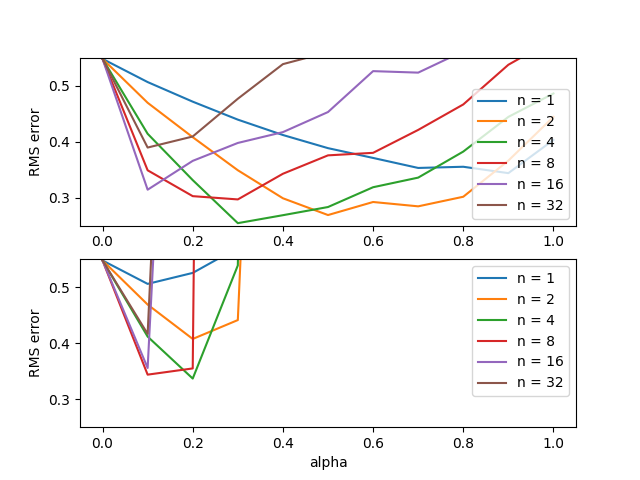
\includegraphics[scale=1]{figure_7_2}

    \subsection{Question}

    Why do you think a larger random walk task (19 states instead of 5) was used in the examples of this chapter?
    Would a smaller walk have shifted the advantage to a different value of n?
    How about the change in left-side outcome from 0 to -1 made in the larger walk?
    Do you think that made any difference in the best value of n?

    \subsection*{Answer}

    If n-step size is close to or bigger than the average number steps to complete an episode then the algorithm approaches to MC which involves variance.
    Using 19 states increases average number of steps to complete an episode thus helps to show how n-step size effects the algorithm.

    If number of states was 5, optimum n-step size would be smaller.
    An empiric study shows that if return value -1 is used with 5 states, most optimum n value would be 1.

    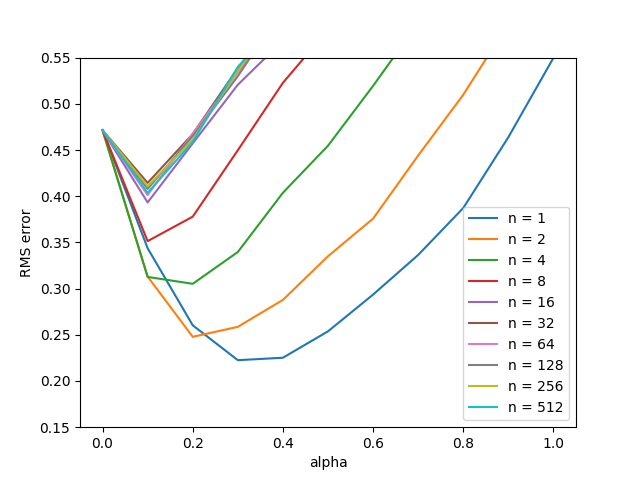
\includegraphics[scale=0.4]{figure_7_3_5states_ret-1}

    Randomwalk with 5 states and reward of 0 on the left, results are found to be different from the -1 case.
    We can interpolate and conclude that changing the return value may affect the result.

    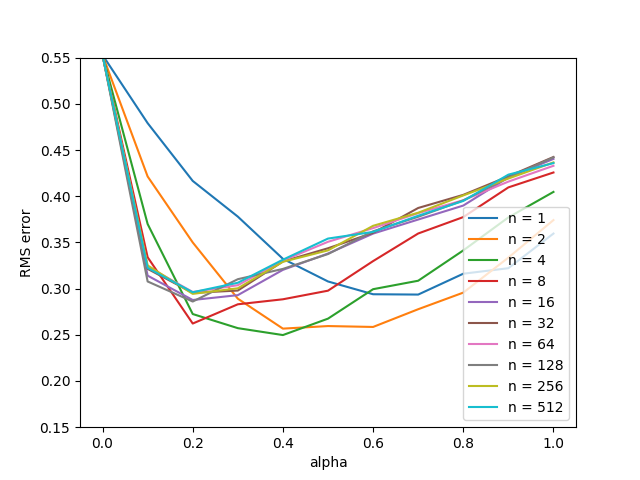
\includegraphics[scale=0.4]{figure_7_3_5states_ret0}

    \subsection{Question}

    Prove that the n-step return of Sarsa (7.4) can be written exactly in terms of a novel TD error.

    \subsection*{Answer}




\end{document}


